
The flux systematic error accounts for the uncertainty one has in
predicting the flux of neutrinos. The uncertainty was propagated using
a code called \texttt{\Gls{JReWeight}} (see instructions and
references in \cite{t2kreweight}), which changes the relative
importance of the selected events based on the neutrino energy and
according to the relative uncertainty as shown in
Figure~\ref{fig:fluxsystematics}. Note that these errors are very
correlated; although there are 100 bins of energy for the neutrino,
after decomposition of the covariance matrix, only seven parameter
eigenvalues are greater than $1\%$, which indicates that the flux
error can been parametrised by only few parameters. These are, by
decreasing order of importance:
\begin{itemize}[noitemsep,topsep=0pt]
\item the proton interaction error, which are constrained by the
  NA61~/~SHINE
  experiments~\cite{Abgrall:2011ae,Abgrall:2011ts,Abgrall:2015hmv},
\item the beam characteristic (profile, intensity, direction) which
  are characterised {\it in situ}, as shown in
  Section~\ref{sec:t2kbeamline},
\item the survey of material around the target station,
\item the horn current and positions.
\end{itemize}

\begin{figure}[ht]
  \center
  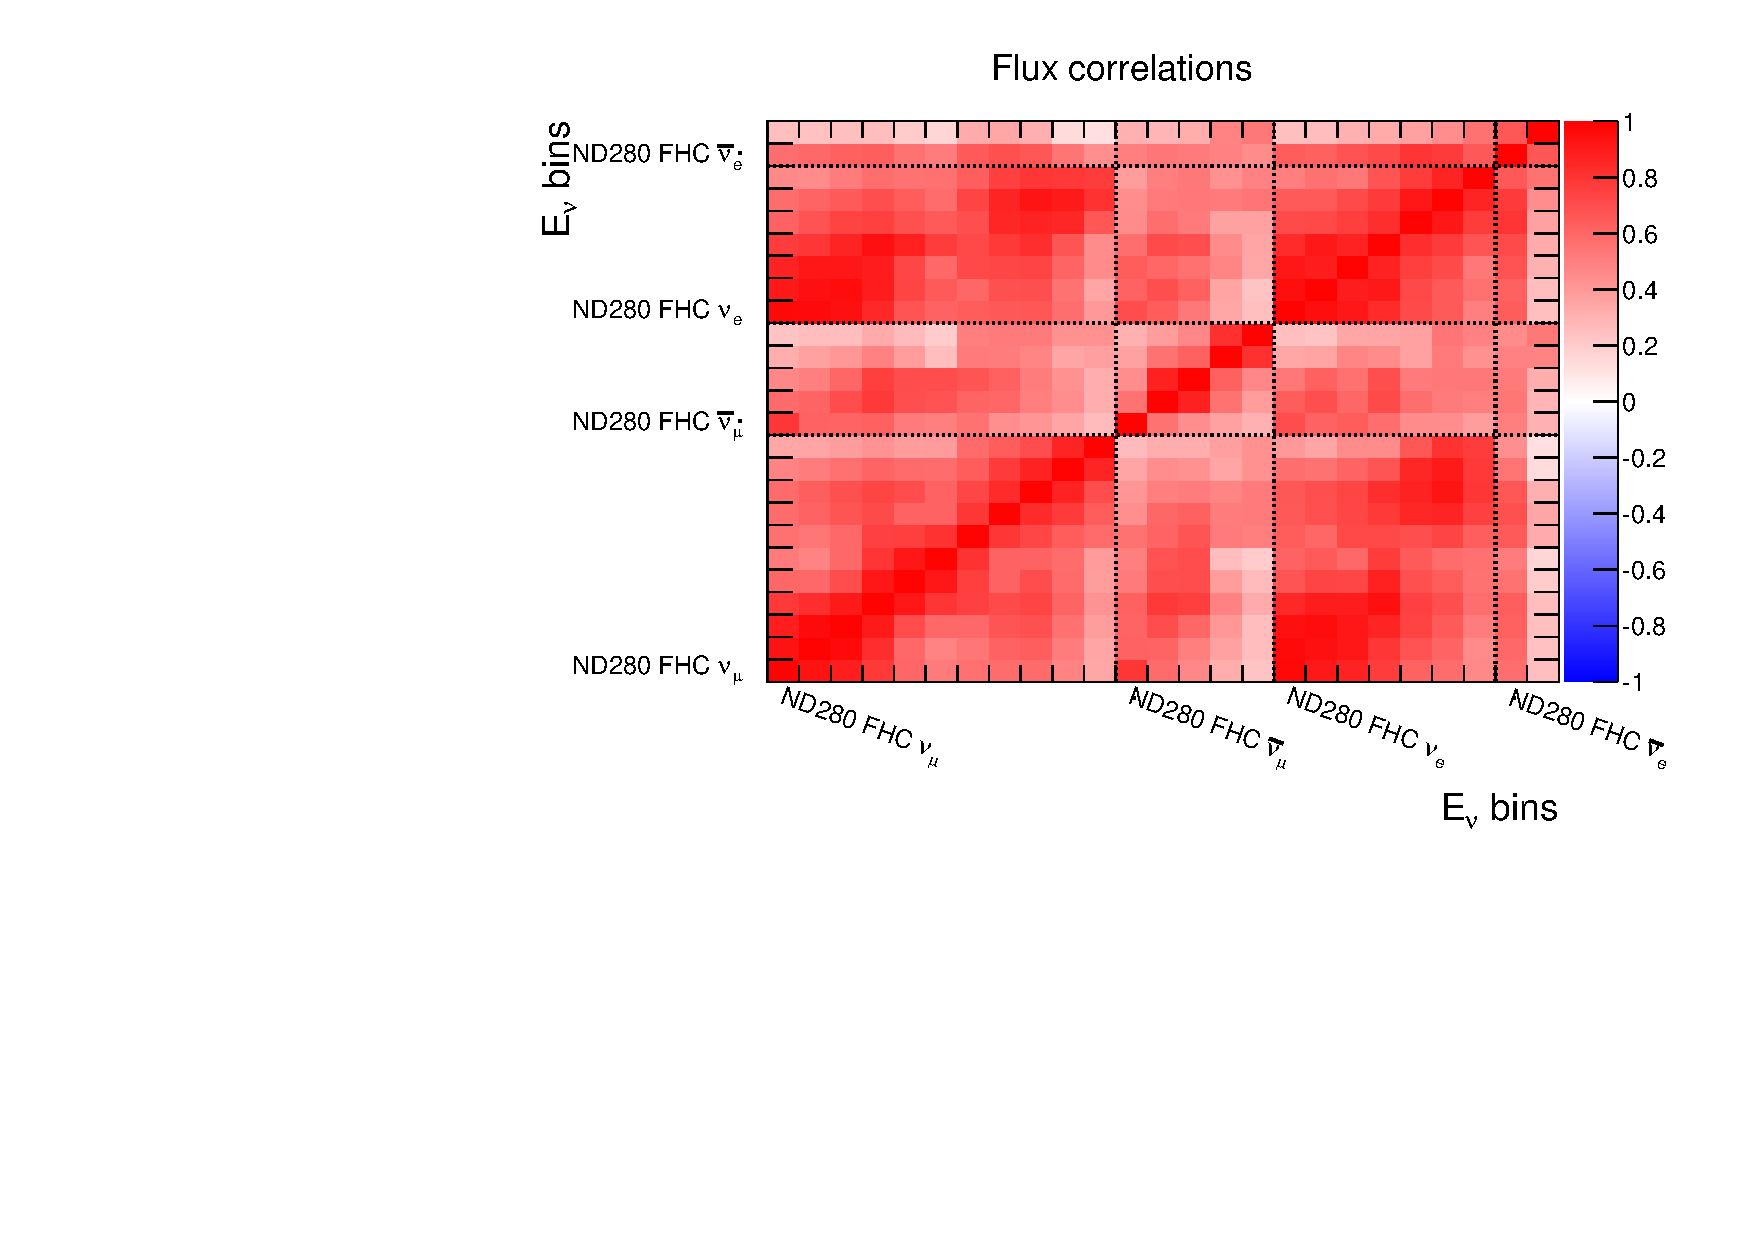
\includegraphics[width=0.8\textwidth]{T2K-TN-254/images/systematics/Flux.pdf} \\
  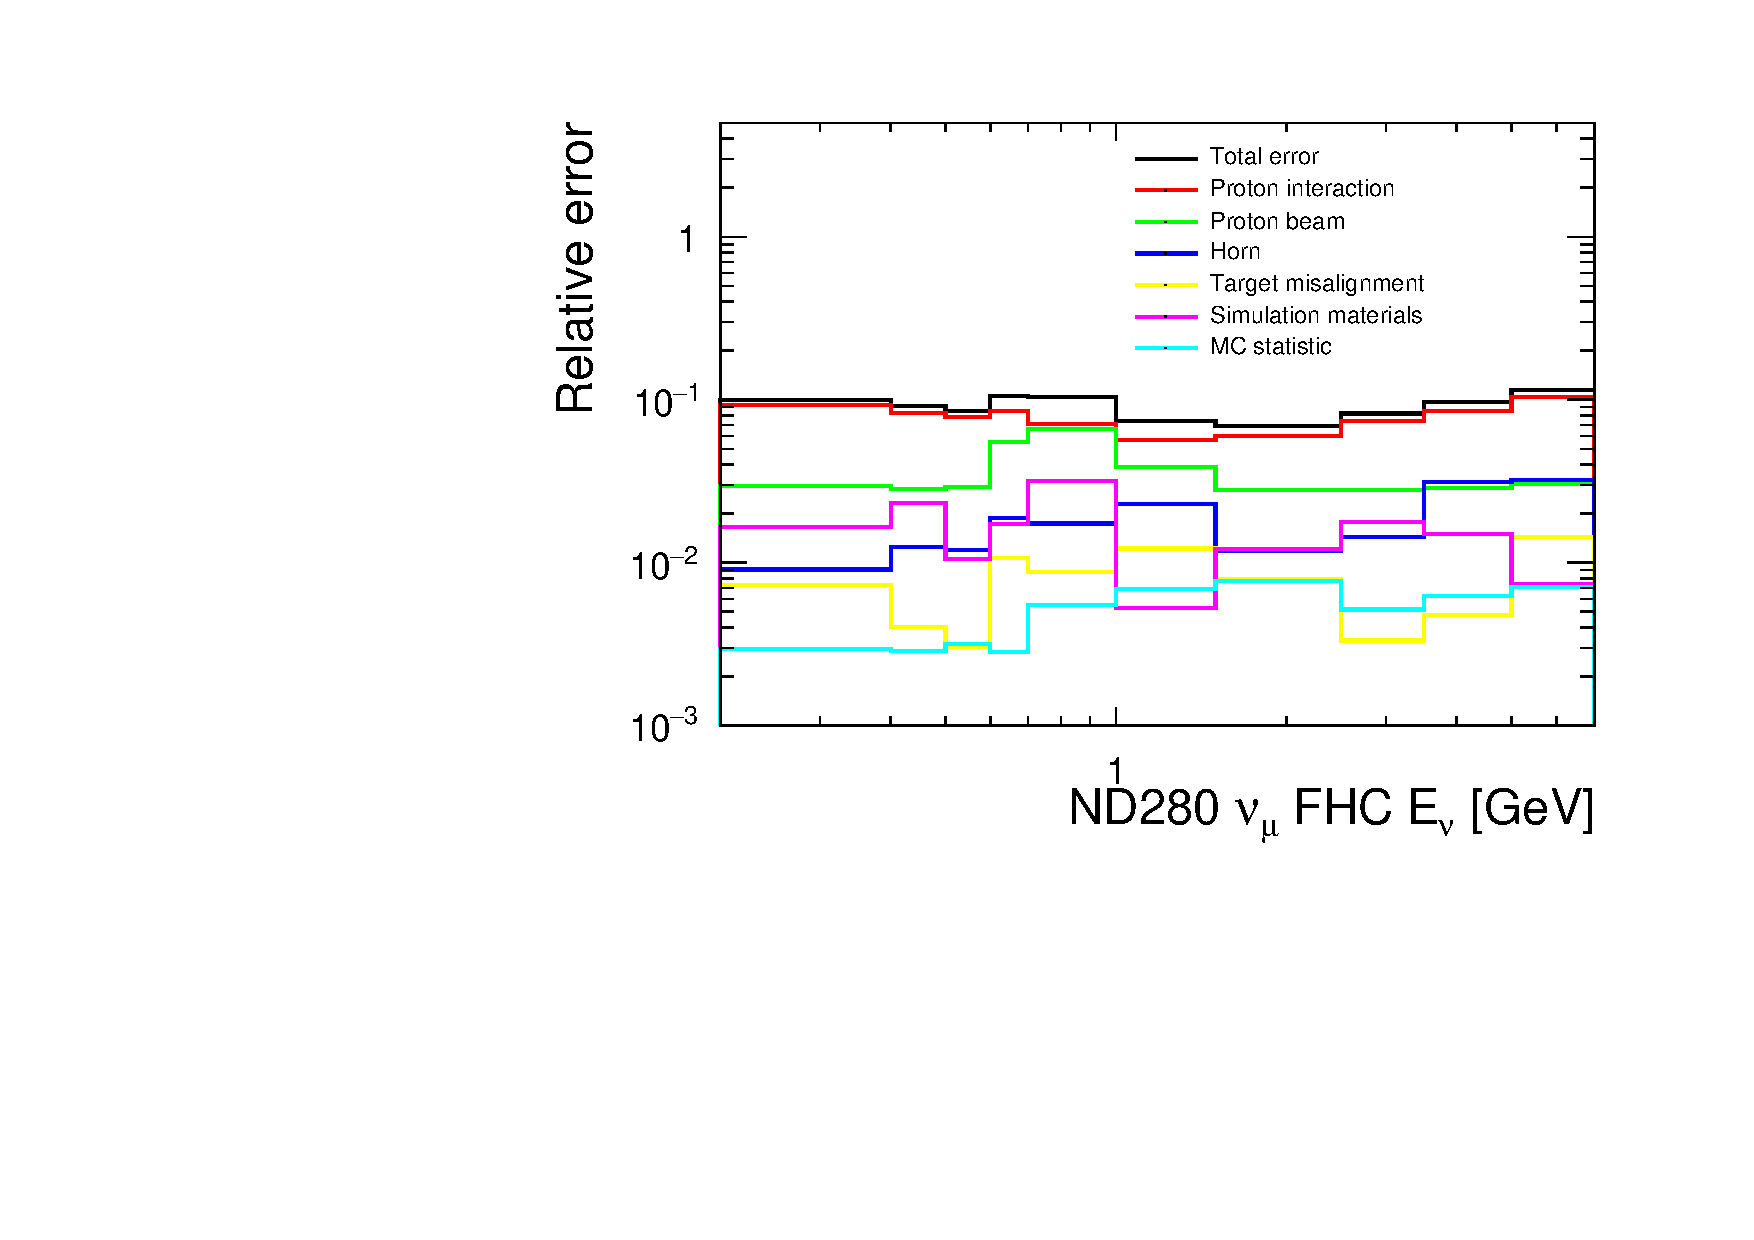
\includegraphics[width=0.8\textwidth]{T2K-TN-254/images/systematics/DiagError.pdf}
  \caption[T2K flux uncertainty and correlations across true energy
  bins in at ND280 and at SK]{\textbf{\textit{Top:}} The \Gls{TK} flux
    uncertainty correlations across true energy bins in for \Gls{ND}
    and \Gls{SK}, while running in \Gls{FHC} and \Gls{RHC} modes, for
    \Gls{numu}, \Gls{anumu}, \Gls{nue} and \Gls{anue}.
    \textbf{\textit{Bottom:}} The diagonal uncertainty for \Gls{numu}
    neutrinos in \Gls{FHC} at the \Gls{ND}. Both extracted from
    \Gls{TK} beam working group
    inputs~\cite{TomislavVladisavljevicFluxTuning2017,MarkHartzFluxUncertainty2017}.}
  \label{fig:fluxsystematics}
\end{figure}

As can be seen in Figure~\ref{fig:fluxsystematics}, the flux
uncertainty is expected to be around $10\%$.

Note that the flux uncertainty was constructed for \Gls{FGD} neutrino
interactions. The photons, on the other hand, can come from regions
far from the \Gls{FGD} central region. Following what was done in
\cite{MarkScott2013}, the conclusion was that the error should not be
increased by more than $5\%$ for \Gls{ECal} interactions. The increase
of the error is considered negligible compared to other effects taken
into account here.

Another motivation for not inflating the flux error is that the
photons do not come from very far from the tracker region, as can be
seen in Appendix~\ref{app:oofvphoton}. The conversion length of the
photons in the \Gls{ECal} ($10.4\text{~cm}$) is much shorter than for
a standard scintillator ($41.1\text{~cm}$), so it is not expected
that the \Gls{OOFV} neutrino interactions come from far regions such
as the \Gls{SMRD}.

The \Gls{PDF} (for Probability Density Function) of the number of
selected events is shown in Figure~\ref{fig:fluxsystematicspdf}.

\begin{figure}[ht]
  \begin{adjustbox}{center}
    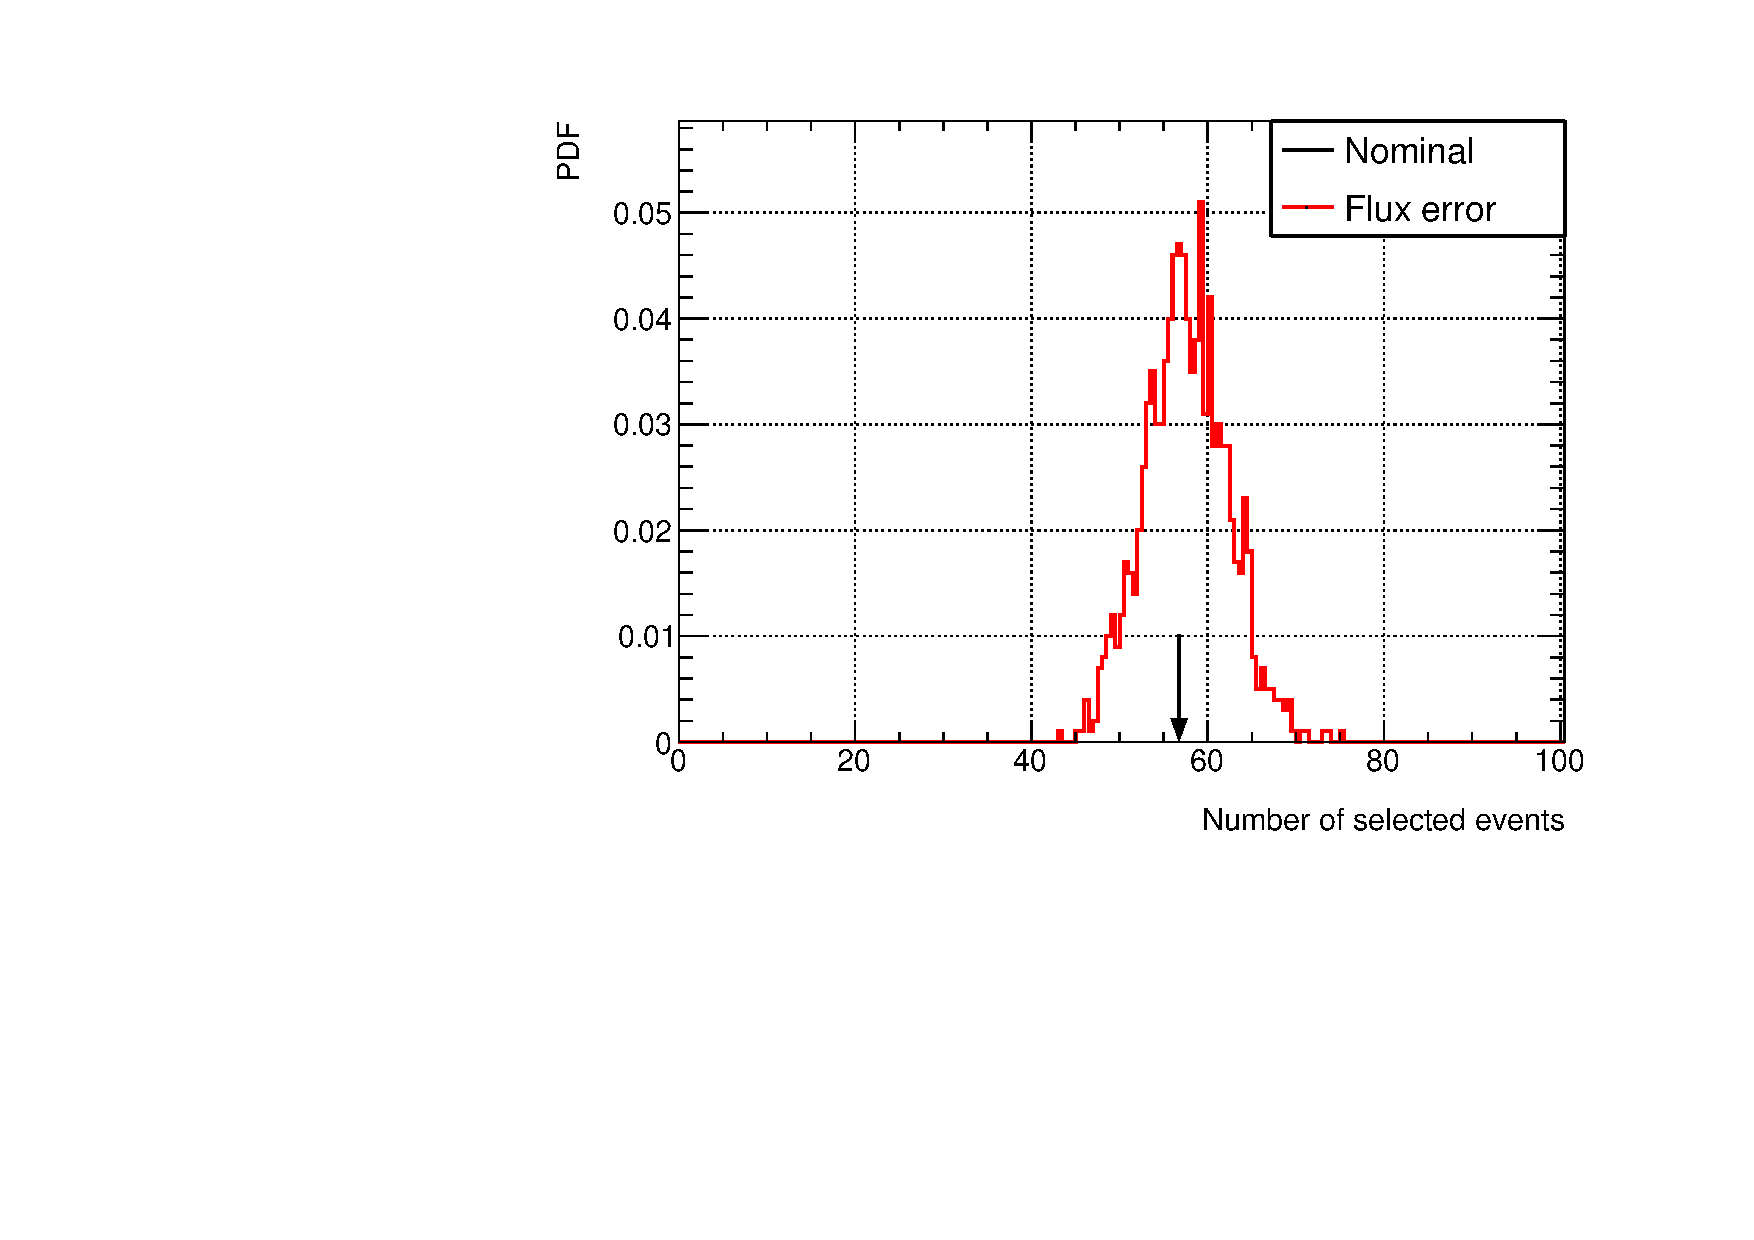
\includegraphics[width=0.8\textwidth]{images/NCg/Flux.pdf} 
  \end{adjustbox}
  \caption[Effect of the flux uncertainty on the number of selected
  events]{Effect of the flux uncertainty on the number of selected
    events. The nominal central value for \Gls{MC} is indicated by the
    arrow.}
  \label{fig:fluxsystematicspdf}
\end{figure}


%%% Local Variables:
%%% mode: latex
%%% TeX-master: "Thesis"
%%% End: